\chapter{近独立粒子系统的统计分布}

统计物理用微观量的统计平均描述宏观性质。给定初态，经典正则方程决定一条轨道，Schrödinger方程决定封闭量子系统的态演化。实验给定的宏观量通常容许大量不同的微观状态，统计计算还需指定这些状态的概率。

% 概率基本知识：概念、互斥事件几率的加法定理、独立事件几率的乘法定理、条件概率、二项分布、Poisson分布、Gauss分布、多个随机变量的联合概率分布、统计平均值和涨落等。

\begin{theorem}
	{Schrödinger方程}{Schrödinger equation}
	对不显含时间的单粒子 Hamilton 算符$\hat H$，能量本征态满足定态Schrödinger方程
	\begin{equation}
		\hat H\ket{n,j} = \varepsilon_n\ket{n,j},
	\end{equation}
	其中$j = 1,\ldots,\omega_n$标记同一能量$\varepsilon_n$的本征子空间的一组正交归一基。

	$\omega_n$称为简并度。当$\omega_n > 1$时，这个能级是简并的。
\end{theorem}

% \begin{example}{一维无穷深势阱}{1-D Infinte Square Potential Well}
% 	一维无穷深势阱能量本征值和简并度
% 	\[
% 		\varepsilon_n=\frac{n^2h^2}{8mL^2},\quad\omega_n=1\quad n=1,2,\ldots.
% 	\]
% 	能级间能量差$\ll$室温下热运动能量(典型值$\qty{25}{meV}$)，
% 	因此能量准连续。
% \end{example}

\begin{definition}
	{微观状态和宏观状态}{microstate and macrostate}
	对本章的近独立粒子系统，用粒子在单粒子态$\ket{i,j}$上的分配来标记计数所用的多体基矢。每一种允许的分配计作一个微观状态(microstate)。
	若只记录各能级$\varepsilon_i$的粒子数，就得到这里采用的宏观状态(macrostate)。

	记分布$\{a_i\}$表示有$a_i$个粒子处于能级$\varepsilon_i$，其对应的微观状态数为$\Omega$。
\end{definition}

\begin{corollary}
	计数时只记录能级占据数$a_i$，一个分布可以对应多种微观分配。例如，当能级简并时，同一能级内还可区分不同的单粒子态$\ket{i,j}$。
\end{corollary}

对于粒子总数$N$、内能$U$和体积$V$确定的平衡态孤立粒子系统，做出两点假设。

\begin{postulate}
	{等概率假设}{equal-probability hypothesis}
	系统的各个微观状态出现的概率相等，即所有分布的总微观状态数$\textstyle\sum_k\Omega_k$的倒数。
\end{postulate}

\begin{remark}
	尽管我们无法直接证明这个假设，但也无从相信某种微观状态更独特，也就是说，我们选取了最简单的均匀分布作为微观状态的先验分布。
\end{remark}

\begin{postulate}
	{最概然分布}{most probable distribution}
	概率最大的分布称为最概然分布(most probable distribution)。当所求宏观量在其附近的相对涨落足够小时，可用这一分布计算平衡值。
\end{postulate}

\begin{corollary}
	基于等概率假设，微观状态数$\Omega$最大的分布即为最概然分布。
\end{corollary}

% \begin{remark}
% 	对于宏观系统，粒子数$N$通常在$10^{23}$量级，在这一量级下，最概然分布与实际分布的相对误差极小。
% \end{remark}

\begin{example}
	{}{}
	考虑两个盒子，$N$个可区分的小球独立地落入左盒或右盒，每个小球落入两盒的概率各为$1/2$。
	我们统计左边盒子中的小球数量$X$作为宏观状态分布。
	$X = k$的分布对应的微观状态数为
	\begin{equation}
		\label{eq:sm-binomial-multiplicity}
		\Omega(X = k) = \binom Nk := \frac{N!}{k!(N - k)!}.
	\end{equation}
	根据等概率假设，$X$服从二项分布，每种分布的概率为
	\[
		\P(X = k) = \frac{\Omega(X = k)}{\sum_{k=0}^N\Omega(X = k)} = \frac1{2^N}\binom Nk.
	\]
	占比$x = X/N$取离散值$k/N$。图中按相邻取值的间距$1/N$将概率质量换算为密度高度$f(k/N) = N\P(X = k)$。分布以$1/2$为中心，标准差为$1/(2\sqrt N)$，大$N$时半高宽也正比于$1/\sqrt N$。
	对于宏观系统，粒子数$N$通常在$\NA \sim 10^{23}$量级，在这一量级下，$X/N$以极高概率落在$1/2$的很小邻域内；这不意味着某个精确取值（例如$X = N/2$）的概率接近1。
	\begin{notecaptionblock}
		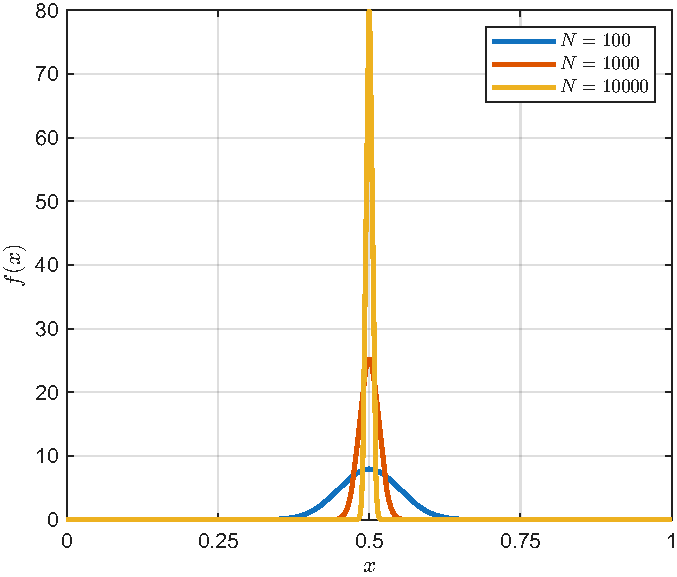
\includegraphics[width=0.6\linewidth]{figures/ML_distribution.pdf}
		\captionof{figure}{分布的概率密度随$N$的变化}
		\label{fig:ML example}
	\end{notecaptionblock}
\end{example}

\section{近独立粒子系统}

\begin{definition}
	{近独立粒子}{nearly independent particle}
	当粒子间相互作用对所研究的平衡性质只产生小修正，可以把多体能量近似写成各粒子能量之和时，称粒子是近独立的(nearly independent)。
\end{definition}

\begin{corollary}
	对于近独立粒子，整个系统的能量可看成单个粒子能量之和，即\eqref{eqn:U=sum a epsilon}。
\end{corollary}

\begin{remark}
	微弱的碰撞可以使能量在粒子间重新分配。在计算平衡能量时可以忽略这种作用，在讨论孤立气体从给定初态趋近平衡的时间时则须考虑它。
\end{remark}

\paragraph{经典分布}

下面首先介绍基于经典力学的经典统计力学中的分布——经典Boltzmann分布。
粒子是可以分辨的，比如一些定域分子(如固体晶格).

\begin{definition}{经典Boltzmann系统}{Boltzmann system}
	性质：粒子可以分辨，量子态容纳粒子数不受限制。

	微观状态数：$N$个粒子全排，除去各能级内$a_i$全排，且能级内可占据$\omega_i$中任一态
	\begin{subequations}
		\label{eqn:Boltzmann system}
		\begin{equation}
			\multiplicity{M} = N!\prod_i\frac{\omega_i^{a_i}}{a_i!}.
		\end{equation}
	\end{subequations}
	其最概然分布称为(经典) Maxwell--Boltzmann分布，满足
	\begin{equation}
		\label{eqn:Boltzmann distribution}
		a_i = \omega_i\e^{-\alpha-\beta\varepsilon_i}.
		\tag{\ref{eqn:Boltzmann system}b}
	\end{equation}
\end{definition}

\begin{proof}
	假设$a_i,\omega_i \gg 1$，
	由Stirling公式，当$x \gg 1$时，
	\begin{equation}
		% \ln x!=x\ln x-x+\frac12\ln x+\frac12\ln(2\pi )+\bigo\biggp{\frac1x}.
		\ln x! = x\ln x - x + \bigo(\ln x).
	\end{equation}
	可得
	\[
		\ln\multiplicity{M} \simeq N\ln N - N + \sum_i a_i\biggb{\ln\biggp{\frac{\omega_i}{a_i}} + 1}.
	\]
	结合粒子数和内能的条件：
	\begin{subequations}
		\begin{align}
			N &= \sum_i a_i,\\
			\label{eqn:U=sum a epsilon}
			U &= \sum_i a_i\varepsilon_i.
		\end{align}
	\end{subequations}
	利用Lagrange乘数法，定义
	\[
		L := \ln\multiplicity{M} + \alpha\Bigp{N - \sum_i a_i} + \beta\Bigp{U - \sum_i a_i\varepsilon_i}.
	\]
	由最概然分布假设，要求
	\[
		\pv L{a_i} = \ln\biggp{\frac{\omega_i}{a_i}} - \alpha - \beta\varepsilon_i = 0
		\implies
		a_i = \omega_i\e^{-\alpha-\beta\varepsilon_i}.
	\]
	验证$\p^2L/\p a_i^2 = -1/a_i < 0$确为极大值点。
\end{proof}

\paragraph{量子分布}

量子粒子与经典粒子是显著不同的，有全同性和自旋两个特点。

\begin{theorem}
	{量子粒子全同性原理}{}
	同种量子粒子是全同的、不可分辨的，交换两个全同粒子的标签不会改变物理状态；不同种粒子则可以区分。
\end{theorem}

\begin{definition}
	{Bose子和Fermi子}{Boson and Fermion}
	自旋量子数为整数的粒子称为Bose子(Boson)，半整数的称为Fermi子(Fermion)。
\end{definition}

\begin{theorem}
	{Pauli不相容原理}{Pauli exclusion principle}
	两个全同Fermi子不可能占据同一单粒子量子态。
\end{theorem}

\begin{definition}{Bose系统}{Bose system}
	性质：粒子不可分辨，量子态容纳粒子数不受限制。

	把$a_i$个相同的粒子符号和$\omega_i - 1$个隔板排成一列，隔板间的粒子数依次给出各单粒子态的占据数。各能级的分配数相乘得到
	\begin{subequations}
		\label{eqn:Bose system}
		\begin{equation}
			\multiplicity{B} = \prod_i\binom{a_i + \omega_i - 1}{a_i} = \prod_i\frac{(a_i + \omega_i - 1)!}{a_i!(\omega_i - 1)!}.
		\end{equation}
	\end{subequations}
	最概然分布称为Bose--Einstein分布，满足
	\begin{equation}
		\label{eqn:Bose distribution}
		a_i = \frac{\omega_i}{\e^{\alpha+\beta\varepsilon_i} - 1}.
		\tag{\ref{eqn:Bose system}b}
	\end{equation}
\end{definition}

\begin{proof}
	假设$a_i,\omega_i \gg 1$，
	可得
	\[
		\ln\multiplicity{B} \simeq \sum_i\biggb{a_i\ln\biggp{1 + \frac{\omega_i}{a_i}} + \omega_i\ln\biggp{1 + \frac{a_i}{\omega_i}}}.
	\]
	在最概然分布下，
	\[
		\pv L{a_i} = \ln\biggp{1 + \frac{\omega_i}{a_i}} - \alpha - \beta\varepsilon_i = 0
		\implies
		a_i = \frac{\omega_i}{\e^{\alpha+\beta\varepsilon_i} - 1}.
	\]
	验证$\p^2L/\p a_i^2 = -\omega_i/[a_i(a_i + \omega_i)] < 0$确为极大值点。
\end{proof}

\begin{definition}{Fermi系统}{Fermi System}
	特点：粒子不可分辨，量子态容纳最多一个粒子。

	在能级$i$的$\omega_i$个单粒子态中选取$a_i$个，各放入一个粒子，得到微观状态数
	\begin{subequations}
		\label{eqn:Fermi system}
		\begin{equation}
			\multiplicity{F} = \prod_i\binom{\omega_i}{a_i} = \prod_i\frac{\omega_i!}{a_i!(\omega_i - a_i)!}.
		\end{equation}
	\end{subequations}
	最概然分布称为Fermi--Dirac分布，满足
	\begin{equation}
		\label{eqn:Fermi distribution}
		a_i = \frac{\omega_i}{\e^{\alpha+\beta\varepsilon_i} + 1}.
		\tag{\ref{eqn:Fermi system}b}
	\end{equation}
\end{definition}

\begin{proof}
	假设每个粗粒化能级组均有$a_i \gg 1$且$\omega_i - a_i \gg 1$，以便使用Stirling近似；不要求$a_i \ll \omega_i$，否则会预先排除强简并情形。
	可得
	\[
		\ln\multiplicity{F} \simeq \sum_i\biggb{a_i\ln\biggp{\frac{\omega_i}{a_i} - 1} - \omega_i\ln\biggp{1 - \frac{a_i}{\omega_i}}}.
	\]
	在最概然分布下，
	\[
		\pv L{a_i} = \ln\biggp{\frac{\omega_i}{a_i} - 1} - \alpha - \beta\varepsilon_i = 0
		\implies
		a_i = \frac{\omega_i}{\e^{\alpha+\beta\varepsilon_i} + 1}.
	\]
	验证$\p^2L/\p a_i^2 = -\omega_i/[a_i(\omega_i - a_i)] < 0$确为极大值点。
\end{proof}

\begin{definition}
	{半经典Boltzmann分布}{semi-classical distribution}

	当各单粒子态的平均占据数均远小于1时，忽略交换修正，Bose分布和Fermi分布都趋于半经典的(semi-classical) Boltzmann分布，其统计权重和占据数为
	\begin{subequations}
		\begin{gather}
			\multiplicity{S} = \prod_i\frac{\omega_i^{a_i}}{a_i!},\\
			a_i = \omega_i\e^{-\alpha-\beta\varepsilon_i}.
		\end{gather}
	\end{subequations}
	条件$a_i \ll \omega_i$称为非简并条件(non-degenerate condition)。取单粒子基态能量为零且$T > 0$时，它等价于$\e^\alpha \gg 1$。
\end{definition}

% \begin{proof}
% 	\[
% 		\ln\multiplicity{S}=\sum_i a_i\ln\omega_i-\ln a_i!
% 		=N+\sum_i a_i\ln\biggp{\frac{\omega_i}{a_i}}.
% 	\]
% \end{proof}

\begin{remark}
	全同粒子的半经典统计权重等于可分辨粒子计数除以$N!$。在固定$N$时，这个因子对所有分布相同，不影响最概然分布。
\end{remark}

\begin{notecaptionblock}
	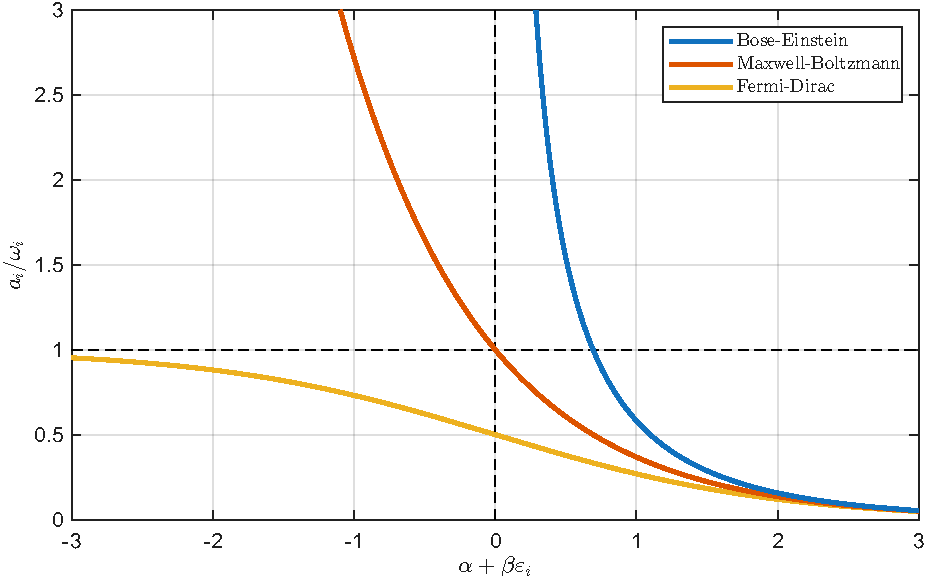
\includegraphics[width=0.8\linewidth]{figures/Boltzmann_Bose_Fermi.pdf}
	\captionof{figure}{三种分布的比较}
	\label{fig:Boltzmann Bose Fermi}
\end{notecaptionblock}

\paragraph{最概然方法误差估计}

对Boltzmann统计，考虑满足$\textstyle \sum_i\vd a_i = 0$、$\textstyle \sum_i\varepsilon_i\vd a_i = 0$的涨落。写成$a_i = a_{i,\mostprobable}(1 + \delta_i)$，其中$\delta_i = \vd a_i/a_{i,\mostprobable}$。在Stirling近似下，$\ln\Omega$的一阶变化为
\[
	\sum_i(\alpha + \beta\varepsilon_i)\vd a_i = 0.
\]
对每组的$|\delta_i| \ll 1$展开，得到
\begin{equation}
	\label{eq:sm-most-probable-fluctuation-weight}
	\ln\frac{\Omega\{a_i\}}{\Omega\{a_{i,\mostprobable}\}}
	= -\frac12\sum_i a_{i,\mostprobable}\delta_i^2
	+ \bigo\!\left(\sum_i a_{i,\mostprobable}|\delta_i|^3\right).
\end{equation}
若受到扰动的能级组总共含有量级为$N \sim 10^{23}$的粒子，且各组相对偏差的绝对值约为$10^{-4}$，则该分布相对于最概然分布的权重已极小：
\[
	\frac{\Omega\{a_i\}}{\Omega\{a_{i,\mostprobable}\}} \simeq \exp\biggp{-\frac12\sum_ia_{i,\mostprobable} \cdot \frac{\vd a_i^2}{a_{i,\mostprobable}^2}} \sim \e^{-10^{23-8}}\lll 1.
\]

\section{宏观量的统计表达式}

\begin{definition}{配分函数}{partition function}
	对于(半)经典Boltzmann分布，定义单粒子配分函数(partition function)
	\begin{equation}
		Z := \sum_i\omega_i\e^{-\beta\varepsilon_i}.
	\end{equation}
	% 单粒子能级$\varepsilon_i$是外参量$y$的函数。
\end{definition}

\begin{corollary}
	配合已知的单粒子能谱，可由配分函数求出占据数、内能和广义力：
	\begin{subequations}
		\begin{align}
			N &= \e^{-\alpha}Z,\\
			% \alpha&=\ln\frac ZN,\\
			\label{eqn:U=-NplnZ}
			U &= -N\pv{\ln Z}\beta,\\
			\label{eqn:Y=-NplnZ/beta}
			Y_k &= -\frac N\beta\pv{\ln Z}{y_k}.
		\end{align}
	\end{subequations}
\end{corollary}

\begin{proof}
	粒子数
	\[
		N = \sum_i a_i = \sum_i \omega_i\e^{-\alpha-\beta\varepsilon_i} = \e^{-\alpha}Z
		\implies \e^{-\alpha} = \frac NZ.
	\]
	内能
	\[
		U = \sum_i a_i\varepsilon_i = \e^{-\alpha}\sum_i \omega_i\varepsilon_i\e^{-\beta\varepsilon_i} = -\frac NZ\pv Z\beta = -N\pv{\ln Z}\beta.
	\]
	对粒子数固定的一系列平衡态，内能的微分为
	\[
		\d U = \sum_i a_i\d\varepsilon_i + \sum_i \varepsilon_i\d a_i
	\]
	前者是粒子分布不变时能级改变导致的内能变化，对应功$\vd W$；
	后者是能级不变时粒子分布改变导致的内能变化，对应热量$\vd Q$。
	故
	\[
		\sum_k Y_k\d y_k = \vd W = \sum_i a_i\d\varepsilon_i = \sum_i a_i\sum_k\pv{\varepsilon_i}{y_k}\d y_k.
	\]
	可得
	\[
		Y_k = \sum_i a_i\pv{\varepsilon_i}{y_k} = \sum_i \omega_i\e^{-\alpha-\beta\varepsilon_i}\pv{\varepsilon_i}{y_k} = -\frac N\beta\pv{\ln Z}{y_k}.
		\qedhere
	\]
\end{proof}

\begin{theorem}{Boltzmann关系}{Boltzmann relation}
	若指定宏观条件下有$\Omega$个等概率的微观态，则熵为
	\begin{equation}
		S = \kB\ln\Omega.
	\end{equation}
	其中$\kB = \qty{1.380649e-23}{\joule\per\kelvin}$为Boltzmann常数。
\end{theorem}

\begin{proof}
	等概率时，将$p_s = 1/\Omega$代入统计熵$\textstyle -\kB\sum_s p_s\ln p_s$即得此式。也可以在Boltzmann分布中直接与热力学的熵比较。固定$N$，有
	\begin{align*}
		N\d\ln Z &= N\biggp{\pv{\ln Z}\beta\d\beta + \sum_k\pv{\ln Z}{y_k}\d y_k} = -U\d\beta - \beta\sum_k Y_k\d y_k\\
		&= -U\d\beta - \beta(\d U - T\d S) = -\d(\beta U) + \beta T\d S.
	\end{align*}
	可得$\d S = \d(N\ln Z + \beta U)/\beta T$，
	将理想气体的统计结果与热力学温标比较，可确定$\beta = 1/(\kB T)$；这不能仅由两边均为全微分推出。于是可得
	\begin{align*}
		S &= S_0 + \kB(N\ln N + \alpha N + \beta U)
		= S_0 + \kB\biggp{N\ln N + \sum_i a_i(\alpha + \beta\varepsilon_i)}\\
		&= S_0 + \kB\biggp{N\ln N + \sum_i a_i\ln\biggp{\frac{\omega_i}{a_i}}}
		\simeq S_0 + \kB\ln\multiplicity{M}.
		\qedhere
	\end{align*}
\end{proof}

\begin{remark}
	上面固定了$N$，积分常数可以依赖$N$。对可分辨粒子取$S_0 = 0$，最后一步对最概然分布的态数使用了Stirling近似。若只给定总能量和粒子数，还须把能壳内各个分布的态数相加。在最概然方法适用的热力学极限中，这个求和与最大项给出相同的熵的广延主项。

	对于全同粒子的半经典气体，置换因子给出$S_0 = -\kB\ln N!$。保留热力学极限的主项时，
	\[
		S \simeq \kB\ln\multiplicity{S} = \kB\ln\biggp{\frac{\multiplicity{M}}{N!}}
		\simeq \kB\biggp{N + \sum_i a_i\ln\biggp{\frac{\omega_i}{a_i}}}.
	\]
\end{remark}

% \begin{corollary}
% 	其他宏观量也可以表示，自由能和化学势
% 	\begin{subequations}
% 		\begin{align}
% 			F&=U-TS=-N\kB T(\alpha+\ln N)-TS_0=
% 			\begin{cases}
% 				-N\kB T(\alpha+\ln N),&\text{classical}\\
% 				-N\kB T\alpha,&\text{semi-classical}
% 			\end{cases}
% 			\\
% 			\mu&=\pvat{F}{N}{T}=-\alpha\kB T.
% 		\end{align}
% 	\end{subequations}
% \end{corollary}

\section{单粒子态的半经典描述}

由理论力学内容，系统的Hamilton量$H \equiv \varepsilon$，广义坐标$q_i$与广义动量$p_i$有关系
\[
	\dot q_i = \pv H{p_i},\quad\dot p_i = -\pv H{q_i}.
\]

\begin{definition}{$\mu$空间}{mu space}
	$\mu$空间是粒子的广义坐标$q_1,\ldots,q_\gamma$与广义动量$p_1,\ldots,p_\gamma$张成的空间。相体积元
	\begin{equation}
		\d\omega = \prod_{i=1}^\gamma\d q_i\nd p_i.
	\end{equation}
	其中$\gamma$为粒子自由度。
\end{definition}

\begin{remark}
	在经典力学中，粒子状态对应$\mu$空间中一个确定的点$(q,p)$。量子力学中，共轭坐标和动量满足$\Delta q_i\Delta p_i \geq \hbar/2$。当一个能量区间内含有许多量子态时，可以用相空间体积估计该区间的态数。
\end{remark}

\begin{theorem}{极限定理}{limit theorem}
	在能谱可作连续近似的半经典极限下，每个平动或轨道量子态平均对应$h^\gamma$的相体积；自旋等内部简并度需另行计入。
\end{theorem}

\begin{corollary}
	由于$(q,p)$是连续的，
	将配分函数写成$\mu$空间中相体积元$\d\omega$的积分形式，
	由极限定理，相体积元$\d\omega$中所含量子态的数量为$\d\omega/h^\gamma$，即
	\begin{equation}
		\label{eq:sm-semiclassical-one-particle-partition}
		Z = \sum_i \omega_i\e^{-\beta\varepsilon_i} \to \int_\mu\frac{\nd\omega}{h^\gamma}\e^{-\beta\varepsilon}.
	\end{equation}
	能量不超过$\varepsilon$的相空间体积记为
	\begin{equation}
		\label{eq:sm-cumulative-phase-volume}
		\Omega(\varepsilon) = \int_{H\leq\varepsilon}\d\omega.
	\end{equation}
	能量区间$(\varepsilon,\varepsilon + \d\varepsilon)$内的轨道量子态数为$g(\varepsilon)\d\varepsilon$，其中态密度为
	\begin{equation}
		g(\varepsilon) = h^{-\gamma}\dv\Omega\varepsilon.
	\end{equation}
	由此可得配分函数$Z$、粒子数$N$和内能$U$的积分表达式
	\begin{subequations}
		\begin{align}
			Z &= \intRplus g(\varepsilon)\e^{-\beta\varepsilon}\d\varepsilon,\\
			N &= \e^{-\alpha}Z = \intRplus g(\varepsilon)\e^{-\alpha-\beta\varepsilon}\d\varepsilon,\\
			U &= -\e^{-\alpha}\pv Z\beta = \intRplus g(\varepsilon)\varepsilon\e^{-\alpha-\beta\varepsilon}\d\varepsilon.
		\end{align}
	\end{subequations}
\end{corollary}

\subsection*{验证极限定理}

\begin{example}{谐振子}{harmonic oscillator}
	一维谐振子的Hamilton量为
	\[
		\varepsilon = \frac{p^2}{2m} + \frac12m\omega^2x^2.
	\]
	考虑能量$\leq \varepsilon$的相空间体积$\Omega(\varepsilon)$，由椭圆面积公式：
	\begin{equation}
		\Omega(\varepsilon) = \int_{\leq\varepsilon}\d\omega = \pi\sqrt{2m\varepsilon}\sqrt{\frac{2\varepsilon}{m\omega^2}} = \frac{2\pi\varepsilon}\omega
		\implies
		g(\varepsilon) = \frac1h\dv\Omega\varepsilon = \frac{2\pi}{h\omega}.
	\end{equation}
	另一方面，量子力学给出谐振子的能量本征值和简并度为
	\[
		\varepsilon_n = \biggp{n + \frac12}\hbar\omega,\quad\omega_n = 1.
	\]
	$\varepsilon_{n-1} \to \varepsilon_n$只有一个状态，
	相体积为$h$
	\[
		\Delta\Omega(\varepsilon_n) = \frac{2\pi}\omega\hbar\omega = h.
	\]
	\tcblower
	二维谐振子的Hamilton量为
	\[
		\varepsilon = \frac{p_x^2 + p_y^2}{2m} + \frac12m\omega^2(x^2 + y^2).
	\]
	由4维单位球体积公式
	\begin{equation}
		\Omega(\varepsilon) = \frac{\pi^2}2 \cdot 2m\varepsilon \cdot \frac{2\varepsilon}{m\omega^2} = \frac{2\pi^2\varepsilon^2}{\omega^2}
		\implies
		g(\varepsilon) = \frac1{h^2 }\dv\Omega\varepsilon = \frac{4\pi^2\varepsilon}{h^2\omega^2}.
	\end{equation}
	另一方面
	\[
		\varepsilon_n = (n + 1)\hbar\omega,\quad\omega_n = n + 1.
	\]
	即$\varepsilon_{n-1} \to \varepsilon_n$有$(n + 1)$个状态，每个状态的
	相体积为
	\[
		\frac{\Delta\Omega(\varepsilon_n)}{n + 1} = \frac{2\pi^2\hbar^2(2n + 1)}{n + 1} \to h^2.
	\]
\end{example}
\begin{example}{转子}{rotor}
	转子的Hamilton量为
	\[
		\varepsilon = \frac1{2I}\biggp{p_\theta^2 + \frac1{\sin^2\theta}p_\phi^2}.
	\]
	其中$I$为转动惯量，
	因此
	\begin{gather}\notag
		\Omega(\varepsilon) = \int\d\theta\nd\phi\int\d p_\theta\nd p_\phi = 2\pi\int_0^\pi\pi\sqrt{2I\varepsilon}\sqrt{2I\varepsilon\sin^2\theta}\d\theta = 8\pi^2I\varepsilon;\\
		\implies
		g(\varepsilon) = \frac1{h^2}\dv\Omega\varepsilon = \frac{8\pi^2I}{h^2}.
	\end{gather}
	另一方面
	\[
		\varepsilon_\ell = \frac{\hbar^2}{2I}\ell(\ell + 1),\quad\omega_\ell = 2\ell + 1.
	\]
	$\varepsilon_{\ell-1} \to \varepsilon_\ell$有$(2\ell + 1)$个状态，每个状态的
	相体积为
	\[
		\frac{\Delta\Omega(\varepsilon_\ell)}{2\ell + 1} = \frac{8\pi^2\hbar^2\ell}{2\ell + 1} \to h^2.
	\]
\end{example}
\begin{example}{单原子分子}{monatomic molecule}
	在非相对论情形下，单原子分子的Hamilton量为
	\[
		\varepsilon = \frac1{2m}(p_x^2 + p_y^2 + p_z^2).
	\]
	在体积为$V$的容器中，
	\begin{gather}\notag
		\Omega(\varepsilon) = V\int_0^{\sqrt{2m\varepsilon}}4\pi p^2\d p = \frac{4\pi V}3(2m\varepsilon)^{3/2};\\
		\implies
		g(\varepsilon) = \frac1{h^3}\dv\Omega\varepsilon = \frac{2\pi V}{h^3}(2m)^{3/2}\sqrt\varepsilon.
	\end{gather}
	若考虑自旋，还应乘自旋因子$g_s = 2s + 1$。

	再从量子数计数。边长为$L$的立方无限深势阱内，$n_x,n_y,n_z$均取正整数，能级为
	\begin{equation}
		\label{eq:sm-cubic-box-spectrum}
		\varepsilon_{n_x,n_y,n_z} = \frac{h^2}{8mL^2}(n_x^2 + n_y^2 + n_z^2),
	\end{equation}
	同一球面上的格点数给出该能级的轨道简并度。球面以内（含球面）的格点数给出截至该能量的累计轨道态数$\mathcal N(\varepsilon)$。球半径远大于格点间距时，用第一卦限内的球体积近似求和，得
	\[
		\mathcal N(\varepsilon) \simeq \frac18 \cdot \frac{4\pi}3\biggp{\frac{8mL^2\varepsilon}{h^2}}^{3/2} = \frac{4\pi V}{3h^3}(2m\varepsilon)^{3/2}.
	\]
	由此得到每个轨道态的平均相体积，并可从累计态数求得相同的半经典态密度：
	\begin{align*}
		\frac{\Omega(\varepsilon)}{\mathcal N(\varepsilon)} &\simeq h^3,\\
		g(\varepsilon) &\simeq \dv{\mathcal N}{\varepsilon}.
	\end{align*}
	\tcblower
	极端相对论情形下
	\[
		\varepsilon = cp = c\sqrt{p_x^2 + p_y^2 + p_z^2}.
	\]
	故
	\begin{equation}
		\Omega(\varepsilon) = V \cdot \frac{4\pi}3\biggp{\frac\varepsilon{c}}^3
		\implies
		g(\varepsilon) = \frac{4\pi V}{h^3c^3}\varepsilon^2.
	\end{equation}
\end{example}
\begin{corollary}
	由\exmref{exm:monatomic molecule} 可知，非相对论情形下
	\[
		\varepsilon = \frac1{2m}\biggp{\frac h{2L}}^2(n_x^2 + n_y^2 + n_z^2) = \frac{h^2}{8m}(n_x^2 + n_y^2 + n_z^2)V^{-2/3}
		\implies
		\pv\varepsilon V = -\frac23\frac\varepsilon V.
	\]
	由\eqref{eqn:Y=-NplnZ/beta}，可得压强
	\begin{equation}
		p = -\sum_i a_i\pv{\varepsilon_i}V = \frac23\sum_i a_i\frac{\varepsilon_i}V = \frac23\frac UV.
	\end{equation}
	而极端相对论情形下
	\[
		\varepsilon = c \cdot \frac h{2V^{1/3}}\sqrt{n_x^2 + n_y^2 + n_z^2}
		\implies
		\pv\varepsilon V = -\frac13\frac\varepsilon V.
	\]
	相似的
	\begin{equation}
		p = \frac13\frac UV.
	\end{equation}
\end{corollary}
